\chapter{Introducción específica} % Main chapter title

\label{Chapter2}

%----------------------------------------------------------------------------------------
%	SECTION 1
%----------------------------------------------------------------------------------------
En este capítulo se describen las tecnologías, herramientas y protocolos utilizados para la realización del trabajo.

\section{Tecnologías de comunicación}
\label{sec:Tecnologías de comunicación}
A continuación se describen los principales protocolos empleados en el trabajo. En la figura \ref{fig:IotProtocols} se observa su posicionamiento en la pila de protocolos para IoT.

\begin{figure}[h]
	\centering
	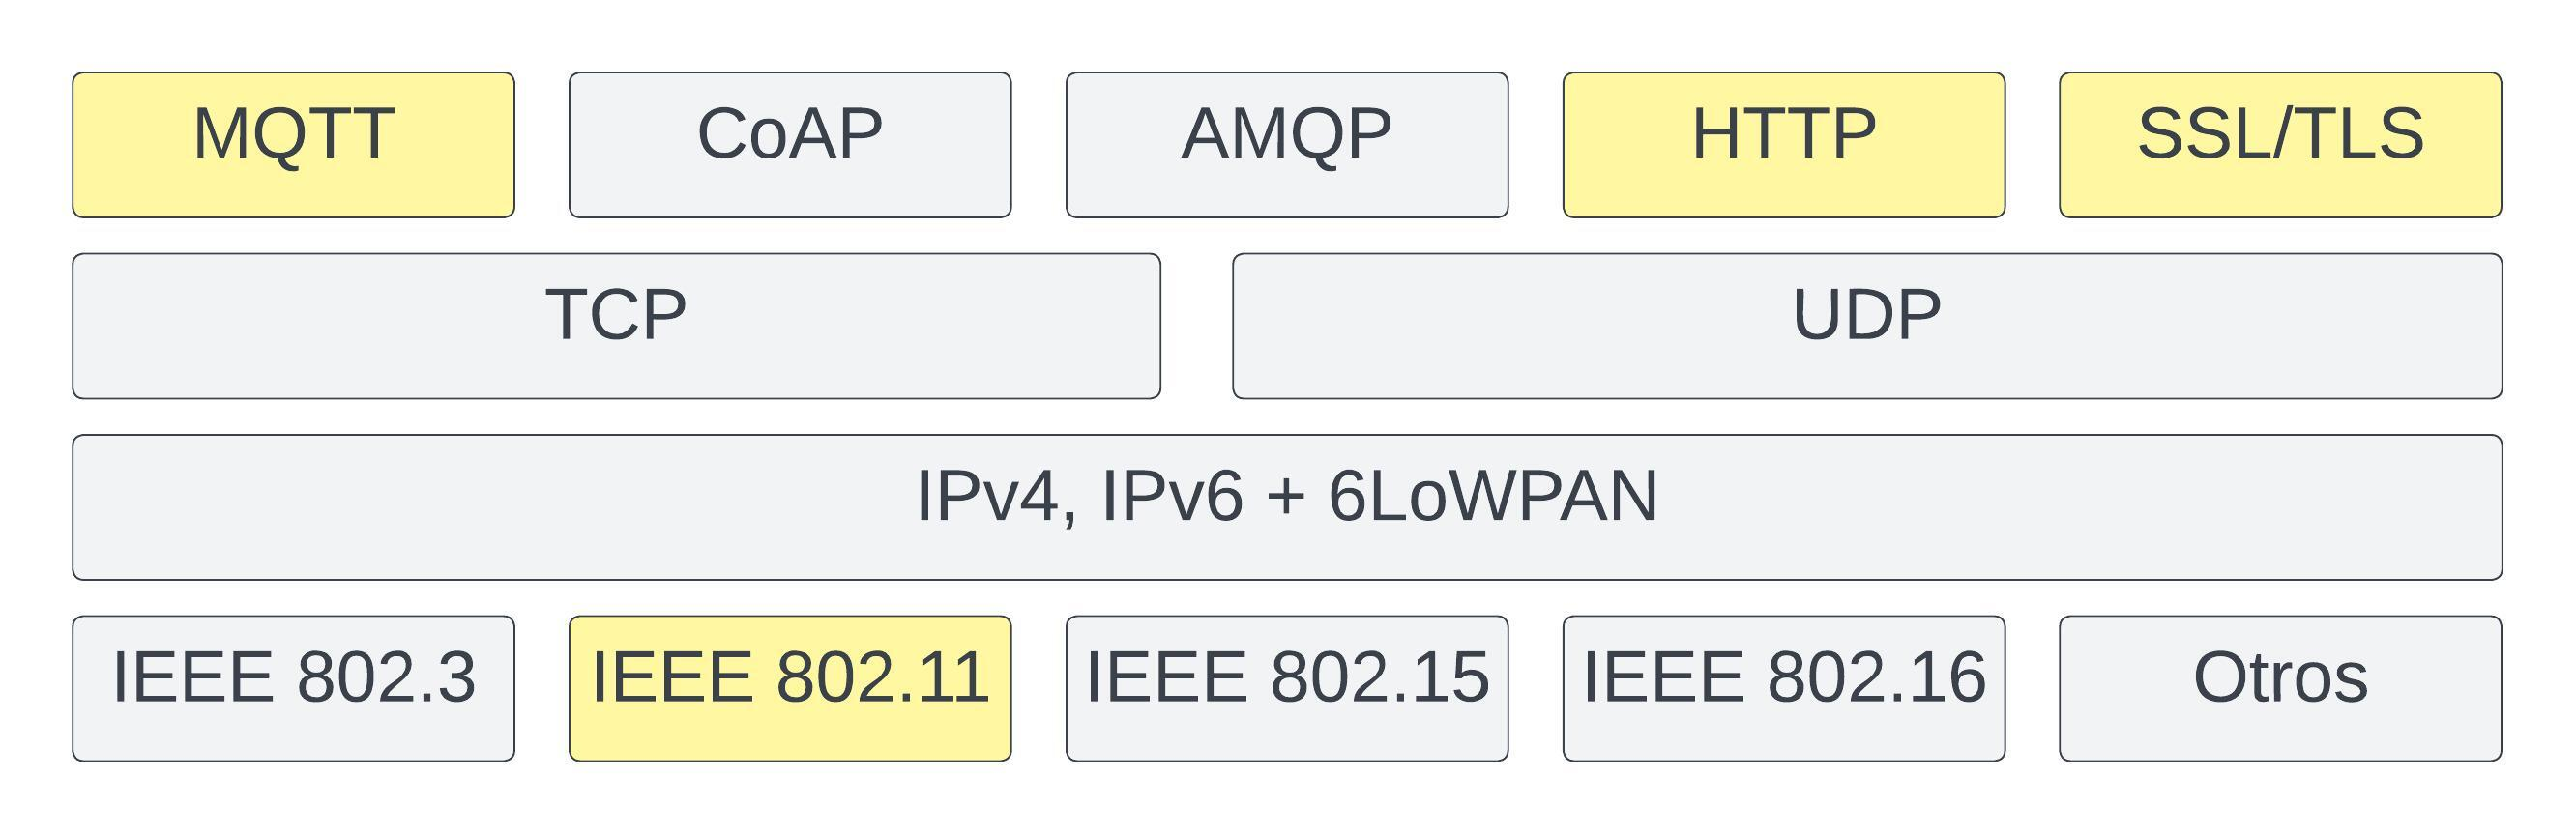
\includegraphics[width=0.75\textwidth]{./Figures/protocols.jpeg}
	\caption[Pila de protocolos para IoT.]{Pila de protocolos para IoT\protect\footnotemark.}
	\label{fig:IotProtocols}

\end{figure}
	\footnotetext{Gráfico creado en base a una imagen tomada de: \citep{8088251}.}

\subsection{Tecnologías Wi-Fi}
\label{sec:Tecnologías Wi-Fi}
El estándar IEEE 802.11 para redes inalámbricas de área local (WLAN) es conocido comercialmente como Wi-Fi. Este estándar presenta dos modos de operación \citep{wifi}
\begin{itemize}
\item Infraestructura: uno o máa \textit{access points} (AP) actúan como puente entre la red cableada y la red inalámbrica. Todas las comunicaciones entre los dispositivos conectados a la red, se realizan a través de los APs. 
\item Ad-hoc: cada nodo puede realizar una conexión directa con otro, sin necesidad de un AP central. Para lograr esto, los nodos se organizan en una red donde todos son capaces de enrutar los paquetes.  
\end{itemize}

\subsection{Protocolo MQTT}
\label{sec:Protocolo MQTT}

El protocolo MQTT fue desarrollado en 1999 con el objetivo principal de crear un protocolo muy eficiente desde el punto de vista del uso del ancho de banda y de muy bajo consumo de energía. Por estas razones es adecuado para el uso en IoT \citep{mqtt:1}.\\
El protocolo MQTT se basa en el paradigma de publicación-suscripción. Este paradigma desvincula un cliente que publica un mensaje o publicador de otros clientes que reciben el mensaje o suscriptores. Sumado a esto, 
MQTT es un protocolo de mensajería asincrónico, lo que significa que no frena al cliente mientras espera por el mensaje. \\ 
Un componente principal del protocolo es el \textit{broker}, su función principal es la de recibir los mensajes de los publicadores y enviarlos  a los clientes suscriptores. Para realizar esta tarea, el \textit{broker} utiliza temas o \textit{topics} para filtrar a los clientes que recibirán el mensaje. De esta manera, el \textit{topic} es un canal virtual que conecta a los publicadores con sus suscriptores \citep{mqtt:1}.

\begin{figure}[h]
	\centering
	\includegraphics[width=0.75\textwidth]{./Figures/mqtt.jpeg}
	\caption[Arquitectura del protocolo MQTT.]{Arquitectura del protocolo MQTT\protect\footnotemark.}
	\label{fig:IotProtocols}

\end{figure}

	\footnotetext{Gráfico creado en base a una imagen tomada de: \citep{mqtt:1}.}


\subsection{Protocolo HTTP}
\label{sec:Protocolo HTTP}

El \textit{Hypertext Transfer Protocol} (HTTP)\citep{http:1} es un protocolo utilizado en la web para el desarrollo de aplicaciones basado en el paradigma cliente-servidor mediante un modelo de \textit{request/response}. En los últimos tiempos se ha asociado a HTTP con la arquitectura REST (\textit{Representational State Transfer})\citep{rest} para facilitar la interacción entre distintas entidades sobre servicios basados en red. Esta asociación permite que los dispositivos interactúen mediante funciones estandares de CRUD (\textit{create, read, update, delete}\citep{10.1145/3292674}. Las funciones de CRUD son mapeadas a los métodos Post, Get, Put y Delete de HTTP respectivamente \citep{GLAROUDIS2020107037}. 

\subsection{Protocolo SSL/TLS}
\label{sec:Protocolo SSL/TLS}
\textit{Secure Socket Layer/Transport Layer Security} (SSL/TLS) \citep{tls:1} es un protocolo criptográfico que proporciona seguridad de extremo a extremo de los datos enviados entre aplicaciones a través de Internet.
TLS evolucionó a partir de \textit{Secure Socket Layers} (SSL), que fue desarrollado originalmente por Netscape Communications Corporation en 1994 para proteger las sesiones web. SSL 1.0 nunca se lanzó públicamente, mientras que SSL 2.0 fue reemplazado rápidamente por SSL 3.0 en el que se basa TLS.\\

Cabe señalar que TLS no protege los datos en los sistemas finales, simplemente asegura la entrega segura de datos a través de Internet, evitando posibles escuchas y/o alteración del contenido.
TLS normalmente se implementa sobre TCP \citep{rfc793} para cifrar los protocolos de la capa de aplicación, como por ejemplo sobre HTTP.

TLS utiliza una combinación de criptografía simétrica y asimétrica, ya que proporciona un buen compromiso entre rendimiento y seguridad cuando se transmiten datos de forma segura \citep{tls:2}. Para mayor seguridad es deseable que un cliente que se conecta a un servidor pueda validar la veracidad de la clave pública del servidor. Esto normalmente se lleva a cabo utilizando un certificado digital X.509 \citep{x509:1} emitido por un tercero de confianza conocido como Autoridad Certificadora (CA) que afirma la autenticidad de la clave pública. En algunos casos, un servidor puede usar un certificado autofirmado en el que el cliente debe confiar explícitamente \citep{tls:2}.

En la figura \ref{fig:ssl2way} se detalla el esquema de autenticación mutua entre dos dispositivos mediante la verificación del certificado presentado.

\begin{figure}[h]
	\centering
	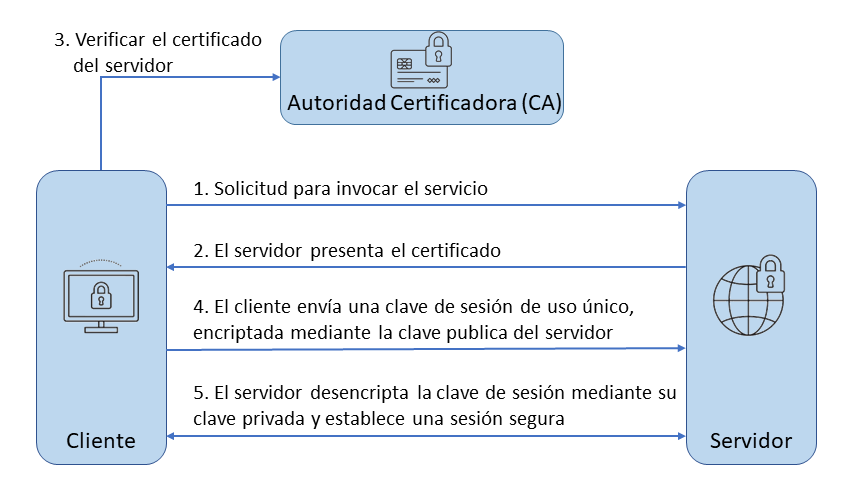
\includegraphics[width=0.75\textwidth]{./Figures/tls.png}
	\caption[Proceso de autenticación de dos vías de SSL.]{Proceso de autenticación de dos vías de SSL\protect\footnotemark.}
	\label{fig:ssl2way}

\end{figure}
	\footnotetext{Gráfico creado en base a una imagen tomada de: https://www.codit.eu/blog/configuring-two-way-ssl-authentication-part-1.}
	
\section{Componentes de hardware utilizado}
\label{sec:Hardware utilizado}

\subsection{Raspberry PI}
\label{sec:Raspberry PI}
La Raspberry Pi es una serie de ordenadores monoplaca u ordenadores de placa simple (SBC por \textit{Single Board Computer}) de bajo costo desarrollados por la Raspberry Pi Foundation \citep{raspberrypi:1}.
Una sus principales características es proveer un conjunto de pines de GPIO (\textit{general purpose input/output} que permiten controlar componentes electrónicos de la computadora física y explorar el Internet de las Cosas.
A pesar de su reducido tamaño, la Raspberry Pi ofrece una capacidad de cómputo comparable a una computadora de escritorio, es por ello que su uso se ha expandido en proyectos que incluyen domótica, \textit{edge computing} \citep{raspberrypi:2}. 

En la tabla \ref{tab:raspberrypi} se listan las principales especificaciones técnicas de la Raspberry Pi modelo 4B
 
\begin{table}[h]
\centering
\caption[Especificaciones técnicas de Raspberry Pi 4B]{Especificaciones técnicas de Raspberry PI 4B}

\begin{tabular}{p{3cm} p{8cm}} 
\toprule
\textbf{Categoría} & \textbf{Especificación}\\

\midrule
Procesador	& Broadcom BCM2711, Quad core Cortex-A72 (ARM v8) 64-bit SoC @ 1.8GHz \\
Memoria SDRAM	 & 1, 2, 4 u 8GB LPDDR4-3200 \\
Wi-Fi	& 2.4 GHz and 5.0 GHz IEEE 802.11ac \\
Bluietooth	&  5.0, BLE \\
Ethernet	& Gigabit, con soporte opcional para POE\\
USB	& 2 puertos  3.0 ; 2 puertos 2.0\\
GPIO	&	Conector de 40 pines\\
HDMI	&  2 puertos micro-HDMI\\
Alimentación	& 5V USB y GPIO\\
Temperatura	& 0 – 50 °C \\
\bottomrule
\hline
\end{tabular}
\label{tab:raspberrypi}
\end{table}
 
\begin{figure}[h]
	\centering
	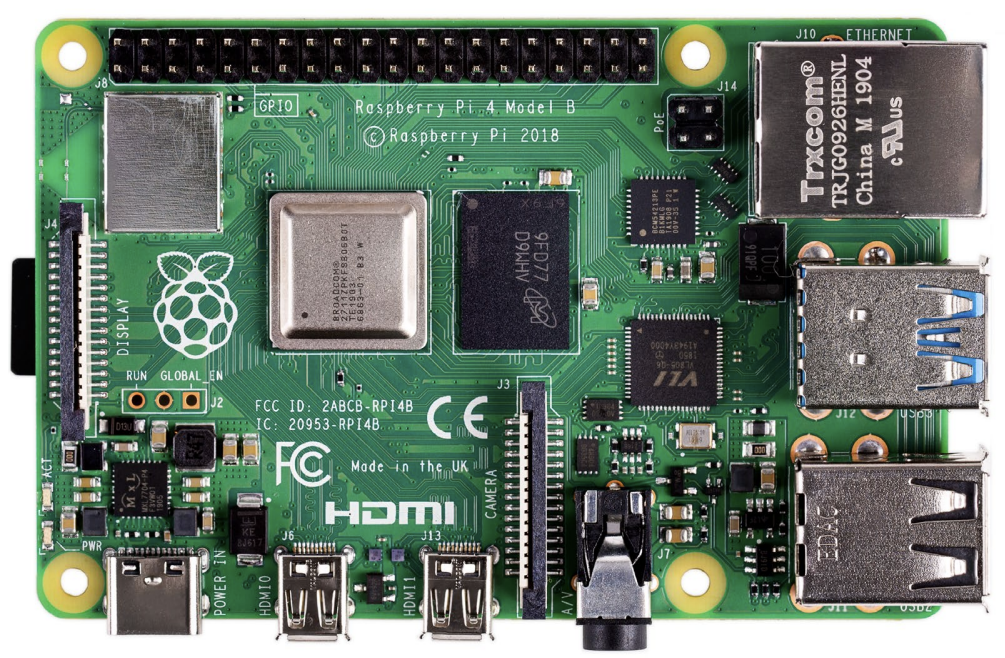
\includegraphics[width=0.75\textwidth]{./Figures/rpi.png}
	\caption[Raspberry PI.]{Raspberry PI\protect\footnotemark.}
	\label{fig:ssl2way}
\footnotetext{Imagen tomada de: https://datasheets.raspberrypi.com/.}
\end{figure}

\subsection{Módulo ESP32}
\label{sec:Módulo ESP32}
ESP32 es una familia de chips SoC (System on a Chip) diseñados para aplicaciones móviles, dispositivos electrónicos portátiles e Internet de las cosas y cuenta con tecnología integrada de Wi-Fi y Bluetooth. El mismo contiene uno o dos microprocesadores Xtensa LX6 de 32 bits de bajo consumo, 448 KB de memoria ROM, 520 KB de memoria SRAM y 16 KB de memoria SRAM en el RTC \citep{esp32}. El ESP32 es desarrollado en Shanghai por la empresa china Espressif Systems y es producido por TSMC usando un proceso de 40 nm.  

\begin{figure}[h]
	\centering
	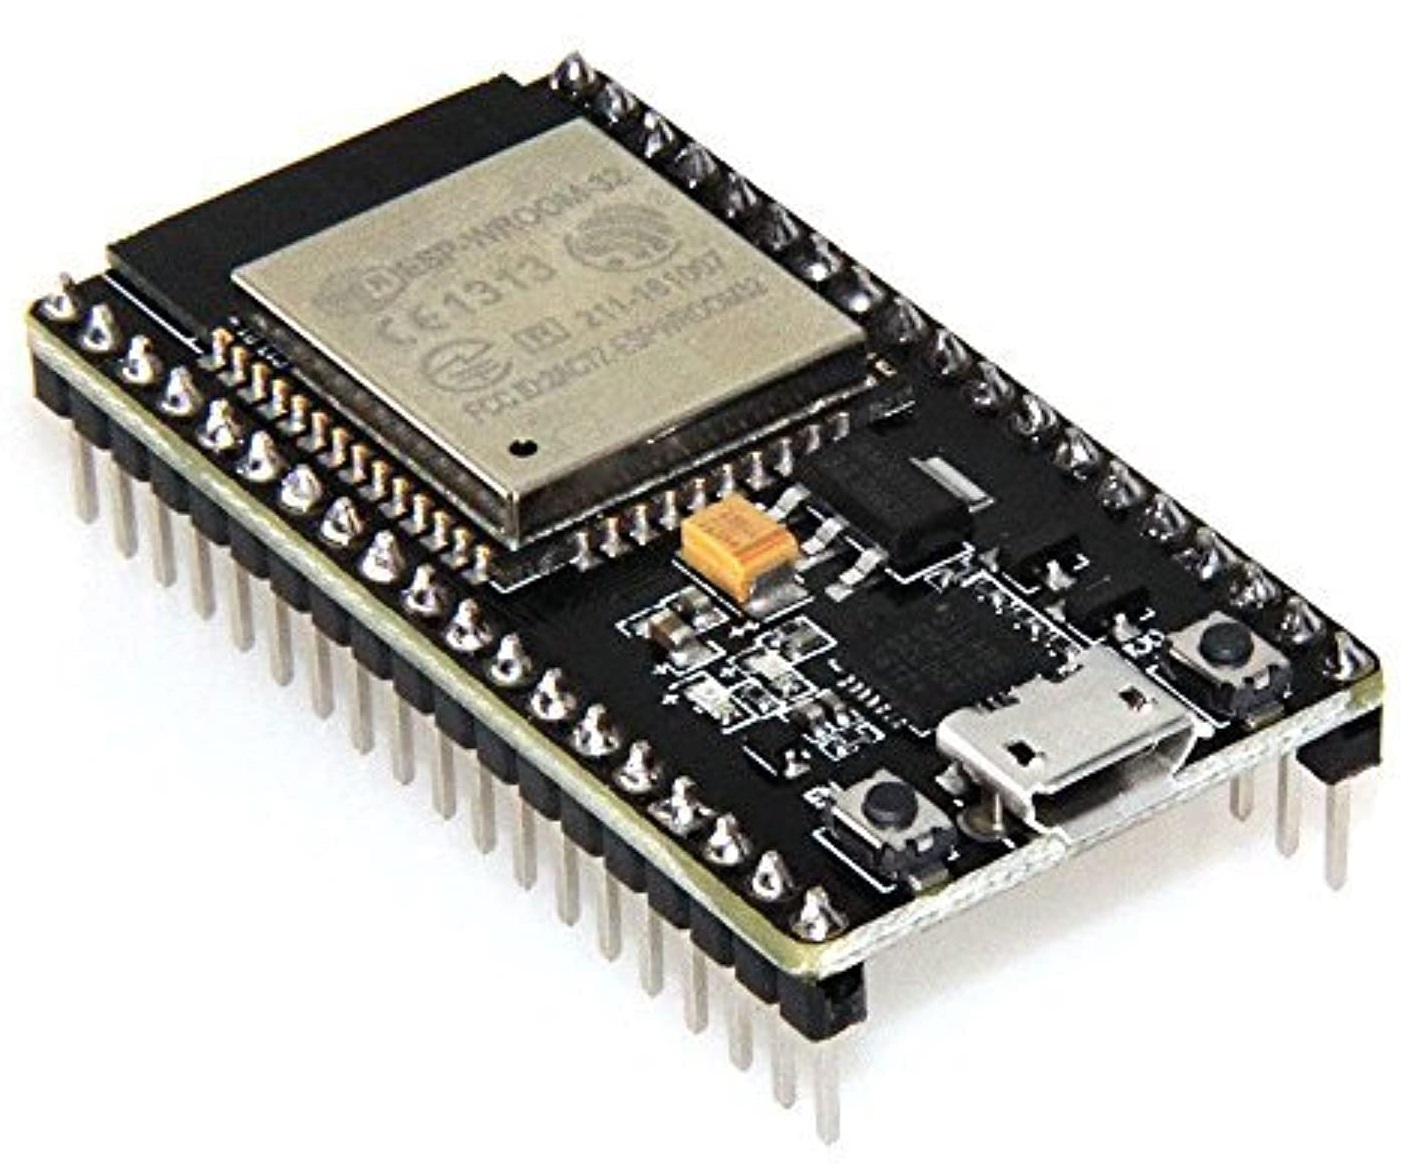
\includegraphics[width=0.30\textwidth]{./Figures/esp32.jpg}
	\caption[Módulo de desarrollo ESP32.]{Módulo de desarrollo ESP32.}
	\label{fig:soilsensor}

\end{figure}

\subsection{Sensores y acturadores}
\label{sec:Sensores y acturadores}
Los siguientes son los principales componentes empleados en los sensores y actuadores del sistema de invernadero inteligente:
\begin{itemize}

\item[] DHT22: es un sensor de temperatura y humedad digital básico y económico. Utiliza un sensor de humedad capacitivo y un termistor para medir el aire circundante y entrega una señal digital en el pin de datos. Funciona con una alimentación de 3,3 a 6 VDC y su rango de medición es de -40 a 80 °C y de 0 a 100 \% de humedad relativa \citep{dht22}.

\item[] Sensor capacitivo de humedad del suelo: es un sensor compuesto de un material resistente a la corrosión, que mide la humedad del suelo indirectamente, por medio de la capacidad observada. Opera con una alimentación de 3,3 a 5,5 VDC.

\item[] Válvula solenoide de dos vías: válvula neumática de un cuarto de pulgada y 12 VDC. Para poder operarla, se utiliza un relé que es un dispositivo electromecánico que funciona como un interruptor controlado por un circuito eléctrico \citep{valve}\citep{rele}.

\end{itemize}
\begin{figure}[h]
	\centering
	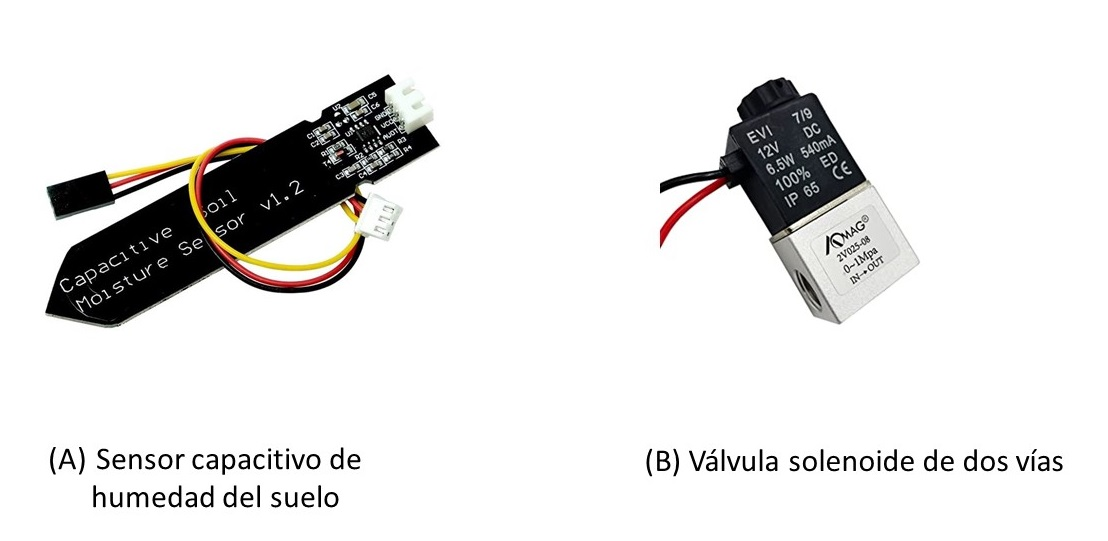
\includegraphics[width=0.90\textwidth]{./Figures/riego.jpg}
	\caption[Dispositivos para control de riego.]{Dispositivos para control de riego.}
	\label{fig:riego}

\end{figure}






\pagebreak
\section{Tecnologías de software aplicadas}
\label{sec:Software aplicado}
\subsection{ThingsBoard}
\label{sec:ThingsBoard}

\subsection{Arduino IDE}
\label{sec:Arduino IDE}



\section{Requerimientos}
\label{sec:Requerimientos}

